\documentclass[1p]{elsarticle_modified}
%\bibliographystyle{elsarticle-num}

%\usepackage[colorlinks]{hyperref}
%\usepackage{abbrmath_seonhwa} %\Abb, \Ascr, \Acal ,\Abf, \Afrak
\usepackage{amsfonts}
\usepackage{amssymb}
\usepackage{amsmath}
\usepackage{amsthm}
\usepackage{scalefnt}
\usepackage{amsbsy}
\usepackage{kotex}
\usepackage{caption}
\usepackage{subfig}
\usepackage{color}
\usepackage{graphicx}
\usepackage{xcolor} %% white, black, red, green, blue, cyan, magenta, yellow
\usepackage{float}
\usepackage{setspace}
\usepackage{hyperref}

\usepackage{tikz}
\usetikzlibrary{arrows}

\usepackage{multirow}
\usepackage{array} % fixed length table
\usepackage{hhline}

%%%%%%%%%%%%%%%%%%%%%
\makeatletter
\renewcommand*\env@matrix[1][\arraystretch]{%
	\edef\arraystretch{#1}%
	\hskip -\arraycolsep
	\let\@ifnextchar\new@ifnextchar
	\array{*\c@MaxMatrixCols c}}
\makeatother %https://tex.stackexchange.com/questions/14071/how-can-i-increase-the-line-spacing-in-a-matrix
%%%%%%%%%%%%%%%

\usepackage[normalem]{ulem}

\newcommand{\msout}[1]{\ifmmode\text{\sout{\ensuremath{#1}}}\else\sout{#1}\fi}
%SOURCE: \msout is \stkout macro in https://tex.stackexchange.com/questions/20609/strikeout-in-math-mode

\newcommand{\cancel}[1]{
	\ifmmode
	{\color{red}\msout{#1}}
	\else
	{\color{red}\sout{#1}}
	\fi
}

\newcommand{\add}[1]{
	{\color{blue}\uwave{#1}}
}

\newcommand{\replace}[2]{
	\ifmmode
	{\color{red}\msout{#1}}{\color{blue}\uwave{#2}}
	\else
	{\color{red}\sout{#1}}{\color{blue}\uwave{#2}}
	\fi
}

\newcommand{\Sol}{\mathcal{S}} %segment
\newcommand{\D}{D} %diagram
\newcommand{\A}{\mathcal{A}} %arc


%%%%%%%%%%%%%%%%%%%%%%%%%%%%%5 test

\def\sl{\operatorname{\textup{SL}}(2,\Cbb)}
\def\psl{\operatorname{\textup{PSL}}(2,\Cbb)}
\def\quan{\mkern 1mu \triangleright \mkern 1mu}

\theoremstyle{definition}
\newtheorem{thm}{Theorem}[section]
\newtheorem{prop}[thm]{Proposition}
\newtheorem{lem}[thm]{Lemma}
\newtheorem{ques}[thm]{Question}
\newtheorem{cor}[thm]{Corollary}
\newtheorem{defn}[thm]{Definition}
\newtheorem{exam}[thm]{Example}
\newtheorem{rmk}[thm]{Remark}
\newtheorem{alg}[thm]{Algorithm}

\newcommand{\I}{\sqrt{-1}}
\begin{document}

%\begin{frontmatter}
%
%\title{Boundary parabolic representations of knots up to 8 crossings}
%
%%% Group authors per affiliation:
%\author{Yunhi Cho} 
%\address{Department of Mathematics, University of Seoul, Seoul, Korea}
%\ead{yhcho@uos.ac.kr}
%
%
%\author{Seonhwa Kim} %\fnref{s_kim}}
%\address{Center for Geometry and Physics, Institute for Basic Science, Pohang, 37673, Korea}
%\ead{ryeona17@ibs.re.kr}
%
%\author{Hyuk Kim}
%\address{Department of Mathematical Sciences, Seoul National University, Seoul 08826, Korea}
%\ead{hyukkim@snu.ac.kr}
%
%\author{Seokbeom Yoon}
%\address{Department of Mathematical Sciences, Seoul National University, Seoul, 08826,  Korea}
%\ead{sbyoon15@snu.ac.kr}
%
%\begin{abstract}
%We find all boundary parabolic representation of knots up to 8 crossings.
%
%\end{abstract}
%\begin{keyword}
%    \MSC[2010] 57M25 
%\end{keyword}
%
%\end{frontmatter}

%\linenumbers
%\tableofcontents
%
\newcommand\colored[1]{\textcolor{white}{\rule[-0.35ex]{0.8em}{1.4ex}}\kern-0.8em\color{red} #1}%
%\newcommand\colored[1]{\textcolor{white}{ #1}\kern-2.17ex	\textcolor{white}{ #1}\kern-1.81ex	\textcolor{white}{ #1}\kern-2.15ex\color{red}#1	}

{\Large $\underline{12a_{1047}~(K12a_{1047})}$}

\setlength{\tabcolsep}{10pt}
\renewcommand{\arraystretch}{1.6}
\vspace{1cm}\begin{tabular}{m{100pt}>{\centering\arraybackslash}m{274pt}}
\multirow{5}{120pt}{
	\centering
	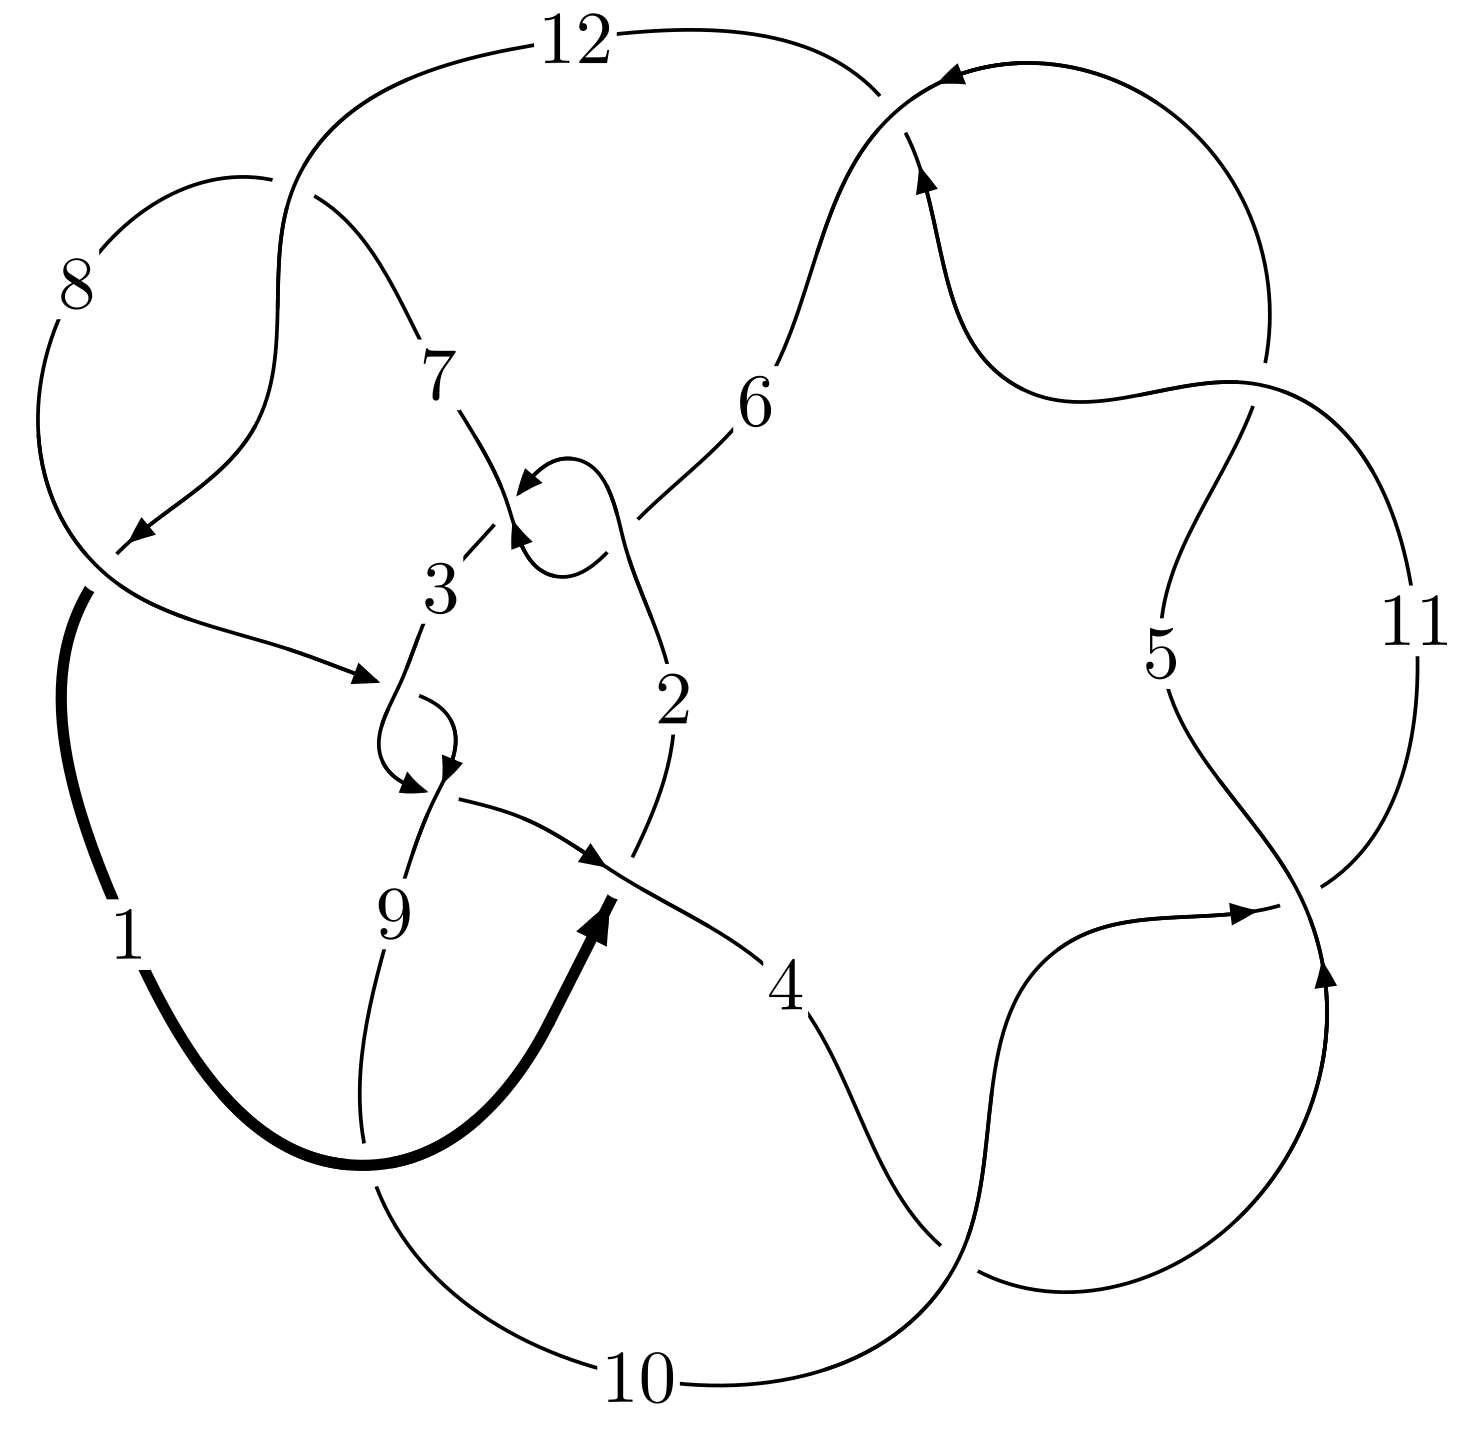
\includegraphics[width=112pt]{../../../GIT/diagram.site/Diagrams/png/1848_12a_1047.png}\\
\ \ \ A knot diagram\footnotemark}&
\allowdisplaybreaks
\textbf{Linearized knot diagam} \\
\cline{2-2}
 &
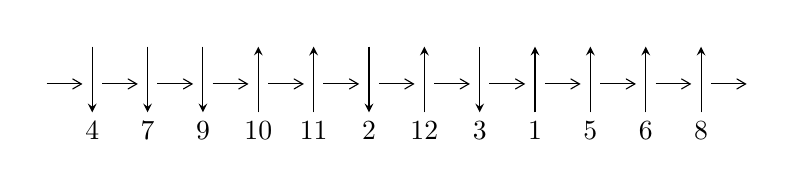
\begin{tikzpicture}[x=20pt, y=17pt]
	% nodes
	\node (C0) at (0, 0) {};
	\node (C1) at (1, 0) {};
	\node (C1U) at (1, +1) {};
	\node (C1D) at (1, -1) {4};

	\node (C2) at (2, 0) {};
	\node (C2U) at (2, +1) {};
	\node (C2D) at (2, -1) {7};

	\node (C3) at (3, 0) {};
	\node (C3U) at (3, +1) {};
	\node (C3D) at (3, -1) {9};

	\node (C4) at (4, 0) {};
	\node (C4U) at (4, +1) {};
	\node (C4D) at (4, -1) {10};

	\node (C5) at (5, 0) {};
	\node (C5U) at (5, +1) {};
	\node (C5D) at (5, -1) {11};

	\node (C6) at (6, 0) {};
	\node (C6U) at (6, +1) {};
	\node (C6D) at (6, -1) {2};

	\node (C7) at (7, 0) {};
	\node (C7U) at (7, +1) {};
	\node (C7D) at (7, -1) {12};

	\node (C8) at (8, 0) {};
	\node (C8U) at (8, +1) {};
	\node (C8D) at (8, -1) {3};

	\node (C9) at (9, 0) {};
	\node (C9U) at (9, +1) {};
	\node (C9D) at (9, -1) {1};

	\node (C10) at (10, 0) {};
	\node (C10U) at (10, +1) {};
	\node (C10D) at (10, -1) {5};

	\node (C11) at (11, 0) {};
	\node (C11U) at (11, +1) {};
	\node (C11D) at (11, -1) {6};

	\node (C12) at (12, 0) {};
	\node (C12U) at (12, +1) {};
	\node (C12D) at (12, -1) {8};
	\node (C13) at (13, 0) {};

	% arrows
	\draw[->,>={angle 60}]
	(C0) edge (C1) (C1) edge (C2) (C2) edge (C3) (C3) edge (C4) (C4) edge (C5) (C5) edge (C6) (C6) edge (C7) (C7) edge (C8) (C8) edge (C9) (C9) edge (C10) (C10) edge (C11) (C11) edge (C12) (C12) edge (C13) ;	\draw[->,>=stealth]
	(C1U) edge (C1D) (C2U) edge (C2D) (C3U) edge (C3D) (C4D) edge (C4U) (C5D) edge (C5U) (C6U) edge (C6D) (C7D) edge (C7U) (C8U) edge (C8D) (C9D) edge (C9U) (C10D) edge (C10U) (C11D) edge (C11U) (C12D) edge (C12U) ;
	\end{tikzpicture} \\
\hhline{~~} \\& 
\textbf{Solving Sequence} \\ \cline{2-2} 
 &
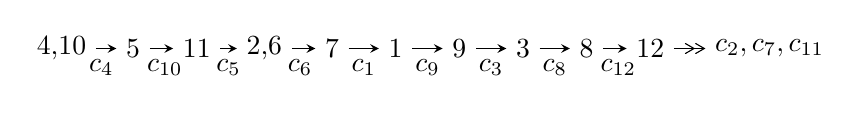
\begin{tikzpicture}[x=23pt, y=7pt]
	% node
	\node (A0) at (-1/8, 0) {4,10};
	\node (A1) at (1, 0) {5};
	\node (A2) at (2, 0) {11};
	\node (A3) at (49/16, 0) {2,6};
	\node (A4) at (33/8, 0) {7};
	\node (A5) at (41/8, 0) {1};
	\node (A6) at (49/8, 0) {9};
	\node (A7) at (57/8, 0) {3};
	\node (A8) at (65/8, 0) {8};
	\node (A9) at (73/8, 0) {12};
	\node (C1) at (1/2, -1) {$c_{4}$};
	\node (C2) at (3/2, -1) {$c_{10}$};
	\node (C3) at (5/2, -1) {$c_{5}$};
	\node (C4) at (29/8, -1) {$c_{6}$};
	\node (C5) at (37/8, -1) {$c_{1}$};
	\node (C6) at (45/8, -1) {$c_{9}$};
	\node (C7) at (53/8, -1) {$c_{3}$};
	\node (C8) at (61/8, -1) {$c_{8}$};
	\node (C9) at (69/8, -1) {$c_{12}$};
	\node (A10) at (11, 0) {$c_{2},c_{7},c_{11}$};

	% edge
	\draw[->,>=stealth]	
	(A0) edge (A1) (A1) edge (A2) (A2) edge (A3) (A3) edge (A4) (A4) edge (A5) (A5) edge (A6) (A6) edge (A7) (A7) edge (A8) (A8) edge (A9) ;
	\draw[->>,>={angle 60}]	
	(A9) edge (A10);
\end{tikzpicture} \\ 

\end{tabular} \\

\footnotetext{
The image of knot diagram is generated by the software ``\textbf{Draw programme}" developed by Andrew Bartholomew(\url{http://www.layer8.co.uk/maths/draw/index.htm\#Running-draw}), where we modified some parts for our purpose(\url{https://github.com/CATsTAILs/LinksPainter}).
}\phantom \\ \newline 
\centering \textbf{Ideals for irreducible components\footnotemark of $X_{\text{par}}$} 
 
\begin{align*}
I^u_{1}&=\langle 
1.72909\times10^{126} u^{87}+4.77505\times10^{125} u^{86}+\cdots+3.37799\times10^{126} b+4.51740\times10^{127},\\
\phantom{I^u_{1}}&\phantom{= \langle  }5.89706\times10^{126} u^{87}-1.19259\times10^{127} u^{86}+\cdots+1.01340\times10^{127} a-3.38574\times10^{128},\;u^{88}- u^{87}+\cdots-39 u-9\rangle \\
I^u_{2}&=\langle 
- u^{13}+10 u^{11}+2 u^{10}-37 u^9-15 u^8+59 u^7+37 u^6-32 u^5-29 u^4-3 u^3-3 u^2+b- u+1,\\
\phantom{I^u_{2}}&\phantom{= \langle  }u^{14}+u^{13}-11 u^{12}-12 u^{11}+45 u^{10}+54 u^9-81 u^8-111 u^7+54 u^6+98 u^5- u^4-23 u^3+4 u^2+a-2 u-3,\\
\phantom{I^u_{2}}&\phantom{= \langle  }u^{15}+2 u^{14}-9 u^{13}-21 u^{12}+25 u^{11}+81 u^{10}-7 u^9-134 u^8-67 u^7+73 u^6+75 u^5+14 u^4- u^3+u^2- u-1\rangle \\
I^u_{3}&=\langle 
b+a+1,\;a^2+a-1,\;u-1\rangle \\
\\
\end{align*}
\raggedright * 3 irreducible components of $\dim_{\mathbb{C}}=0$, with total 105 representations.\\
\footnotetext{All coefficients of polynomials are rational numbers. But the coefficients are sometimes approximated in decimal forms when there is not enough margin.}
\newpage
\renewcommand{\arraystretch}{1}
\centering \section*{I. $I^u_{1}= \langle 1.73\times10^{126} u^{87}+4.78\times10^{125} u^{86}+\cdots+3.38\times10^{126} b+4.52\times10^{127},\;5.90\times10^{126} u^{87}-1.19\times10^{127} u^{86}+\cdots+1.01\times10^{127} a-3.39\times10^{128},\;u^{88}- u^{87}+\cdots-39 u-9 \rangle$}
\flushleft \textbf{(i) Arc colorings}\\
\begin{tabular}{m{7pt} m{180pt} m{7pt} m{180pt} }
\flushright $a_{4}=$&$\begin{pmatrix}1\\0\end{pmatrix}$ \\
\flushright $a_{10}=$&$\begin{pmatrix}0\\u\end{pmatrix}$ \\
\flushright $a_{5}=$&$\begin{pmatrix}1\\- u^2\end{pmatrix}$ \\
\flushright $a_{11}=$&$\begin{pmatrix}u\\- u^3+u\end{pmatrix}$ \\
\flushright $a_{2}=$&$\begin{pmatrix}-0.581911 u^{87}+1.17683 u^{86}+\cdots+115.370 u+33.4098\\-0.511869 u^{87}-0.141358 u^{86}+\cdots-53.8841 u-13.3731\end{pmatrix}$ \\
\flushright $a_{6}=$&$\begin{pmatrix}- u^2+1\\u^4-2 u^2\end{pmatrix}$ \\
\flushright $a_{7}=$&$\begin{pmatrix}0.0734218 u^{87}+0.473497 u^{86}+\cdots+30.4353 u+7.86884\\0.0107578 u^{87}+0.392321 u^{86}+\cdots+19.7593 u+8.34879\end{pmatrix}$ \\
\flushright $a_{1}=$&$\begin{pmatrix}-1.09378 u^{87}+1.03547 u^{86}+\cdots+61.4864 u+20.0368\\-0.511869 u^{87}-0.141358 u^{86}+\cdots-53.8841 u-13.3731\end{pmatrix}$ \\
\flushright $a_{9}=$&$\begin{pmatrix}-0.0591516 u^{87}+0.559425 u^{86}+\cdots-85.4131 u-24.0817\\-0.195623 u^{87}+0.127976 u^{86}+\cdots+17.9905 u+5.97919\end{pmatrix}$ \\
\flushright $a_{3}=$&$\begin{pmatrix}0.734242 u^{87}-0.261255 u^{86}+\cdots+81.8451 u+23.0218\\0.245238 u^{87}-0.171240 u^{86}+\cdots-33.3568 u-11.2988\end{pmatrix}$ \\
\flushright $a_{8}=$&$\begin{pmatrix}-0.225229 u^{87}-0.569456 u^{86}+\cdots-48.8124 u-13.9685\\-0.0267257 u^{87}-0.516094 u^{86}+\cdots-19.8640 u-9.48832\end{pmatrix}$ \\
\flushright $a_{12}=$&$\begin{pmatrix}- u^3+2 u\\u^5-3 u^3+u\end{pmatrix}$\\&\end{tabular}
\flushleft \textbf{(ii) Obstruction class $= -1$}\\~\\
\flushleft \textbf{(iii) Cusp Shapes $= -1.05002 u^{87}+1.35659 u^{86}+\cdots+167.292 u+51.3039$}\\~\\
\newpage\renewcommand{\arraystretch}{1}
\flushleft \textbf{(iv) u-Polynomials at the component}\newline \\
\begin{tabular}{m{50pt}|m{274pt}}
Crossings & \hspace{64pt}u-Polynomials at each crossing \\
\hline $$\begin{aligned}c_{1}\end{aligned}$$&$\begin{aligned}
&u^{88}-2 u^{87}+\cdots-245 u+49
\end{aligned}$\\
\hline $$\begin{aligned}c_{2},c_{6}\end{aligned}$$&$\begin{aligned}
&u^{88}-2 u^{87}+\cdots-288 u+32
\end{aligned}$\\
\hline $$\begin{aligned}c_{3},c_{8}\end{aligned}$$&$\begin{aligned}
&u^{88}+u^{87}+\cdots-46 u+41
\end{aligned}$\\
\hline $$\begin{aligned}c_{4},c_{5},c_{10}\\c_{11}\end{aligned}$$&$\begin{aligned}
&u^{88}- u^{87}+\cdots-39 u-9
\end{aligned}$\\
\hline $$\begin{aligned}c_{7},c_{12}\end{aligned}$$&$\begin{aligned}
&u^{88}+2 u^{87}+\cdots-7 u+1
\end{aligned}$\\
\hline $$\begin{aligned}c_{9}\end{aligned}$$&$\begin{aligned}
&u^{88}-2 u^{87}+\cdots-224 u+64
\end{aligned}$\\
\hline
\end{tabular}\\~\\
\newpage\renewcommand{\arraystretch}{1}
\flushleft \textbf{(v) Riley Polynomials at the component}\newline \\
\begin{tabular}{m{50pt}|m{274pt}}
Crossings & \hspace{64pt}Riley Polynomials at each crossing \\
\hline $$\begin{aligned}c_{1}\end{aligned}$$&$\begin{aligned}
&y^{88}+2 y^{87}+\cdots+155967 y+2401
\end{aligned}$\\
\hline $$\begin{aligned}c_{2},c_{6}\end{aligned}$$&$\begin{aligned}
&y^{88}-50 y^{87}+\cdots-30208 y+1024
\end{aligned}$\\
\hline $$\begin{aligned}c_{3},c_{8}\end{aligned}$$&$\begin{aligned}
&y^{88}-61 y^{87}+\cdots-33850 y+1681
\end{aligned}$\\
\hline $$\begin{aligned}c_{4},c_{5},c_{10}\\c_{11}\end{aligned}$$&$\begin{aligned}
&y^{88}-109 y^{87}+\cdots-4077 y+81
\end{aligned}$\\
\hline $$\begin{aligned}c_{7},c_{12}\end{aligned}$$&$\begin{aligned}
&y^{88}-58 y^{87}+\cdots-165 y+1
\end{aligned}$\\
\hline $$\begin{aligned}c_{9}\end{aligned}$$&$\begin{aligned}
&y^{88}-22 y^{87}+\cdots-111616 y+4096
\end{aligned}$\\
\hline
\end{tabular}\\~\\
\newpage\flushleft \textbf{(vi) Complex Volumes and Cusp Shapes}
$$\begin{array}{c|c|c}  
\text{Solutions to }I^u_{1}& \I (\text{vol} + \sqrt{-1}CS) & \text{Cusp shape}\\
 \hline 
\begin{aligned}
u &= -0.998937\phantom{ +0.000000I} \\
a &= -1.49905\phantom{ +0.000000I} \\
b &= \phantom{-}0.753833\phantom{ +0.000000I}\end{aligned}
 & -4.40347\phantom{ +0.000000I} & \phantom{-0.000000 } 0 \\ \hline\begin{aligned}
u &= \phantom{-}0.854468 + 0.452941 I \\
a &= -0.024901 + 1.322860 I \\
b &= \phantom{-}1.30651 - 1.01094 I\end{aligned}
 & -4.26425 + 6.50157 I & \phantom{-0.000000 } 0 \\ \hline\begin{aligned}
u &= \phantom{-}0.854468 - 0.452941 I \\
a &= -0.024901 - 1.322860 I \\
b &= \phantom{-}1.30651 + 1.01094 I\end{aligned}
 & -4.26425 - 6.50157 I & \phantom{-0.000000 } 0 \\ \hline\begin{aligned}
u &= -0.988389 + 0.302465 I \\
a &= \phantom{-}0.573158 - 0.806046 I \\
b &= \phantom{-}0.516057 + 0.734460 I\end{aligned}
 & \phantom{-}6.01796 - 1.94925 I & \phantom{-0.000000 } 0 \\ \hline\begin{aligned}
u &= -0.988389 - 0.302465 I \\
a &= \phantom{-}0.573158 + 0.806046 I \\
b &= \phantom{-}0.516057 - 0.734460 I\end{aligned}
 & \phantom{-}6.01796 + 1.94925 I & \phantom{-0.000000 } 0 \\ \hline\begin{aligned}
u &= \phantom{-}0.948493 + 0.063667 I \\
a &= \phantom{-}0.752167 + 0.532122 I \\
b &= -0.916241 - 0.735839 I\end{aligned}
 & \phantom{-}2.21145 + 0.85741 I & \phantom{-0.000000 } 0 \\ \hline\begin{aligned}
u &= \phantom{-}0.948493 - 0.063667 I \\
a &= \phantom{-}0.752167 - 0.532122 I \\
b &= -0.916241 + 0.735839 I\end{aligned}
 & \phantom{-}2.21145 - 0.85741 I & \phantom{-0.000000 } 0 \\ \hline\begin{aligned}
u &= -0.878362 + 0.596346 I \\
a &= \phantom{-}0.304863 - 1.160660 I \\
b &= \phantom{-}1.11506 + 0.98368 I\end{aligned}
 & -0.69878 - 13.36100 I & \phantom{-0.000000 } 0 \\ \hline\begin{aligned}
u &= -0.878362 - 0.596346 I \\
a &= \phantom{-}0.304863 + 1.160660 I \\
b &= \phantom{-}1.11506 - 0.98368 I\end{aligned}
 & -0.69878 + 13.36100 I & \phantom{-0.000000 } 0 \\ \hline\begin{aligned}
u &= \phantom{-}0.249913 + 0.895625 I \\
a &= \phantom{-}0.307031 - 0.093746 I \\
b &= -0.084975 - 0.628944 I\end{aligned}
 & \phantom{-}1.56940 - 1.74873 I & \phantom{-0.000000 } 0\\
 \hline 
 \end{array}$$\newpage$$\begin{array}{c|c|c}  
\text{Solutions to }I^u_{1}& \I (\text{vol} + \sqrt{-1}CS) & \text{Cusp shape}\\
 \hline 
\begin{aligned}
u &= \phantom{-}0.249913 - 0.895625 I \\
a &= \phantom{-}0.307031 + 0.093746 I \\
b &= -0.084975 + 0.628944 I\end{aligned}
 & \phantom{-}1.56940 + 1.74873 I & \phantom{-0.000000 } 0 \\ \hline\begin{aligned}
u &= \phantom{-}0.859303 + 0.642777 I \\
a &= -0.350047 - 0.725789 I \\
b &= -0.549384 + 0.933116 I\end{aligned}
 & \phantom{-}3.59516 + 6.91928 I & \phantom{-0.000000 } 0 \\ \hline\begin{aligned}
u &= \phantom{-}0.859303 - 0.642777 I \\
a &= -0.350047 + 0.725789 I \\
b &= -0.549384 - 0.933116 I\end{aligned}
 & \phantom{-}3.59516 - 6.91928 I & \phantom{-0.000000 } 0 \\ \hline\begin{aligned}
u &= \phantom{-}0.834522 + 0.322778 I \\
a &= -0.90185 - 1.49057 I \\
b &= -0.889748 + 0.869352 I\end{aligned}
 & \phantom{-}2.46924 + 6.85078 I & \phantom{-0.000000 } 0 \\ \hline\begin{aligned}
u &= \phantom{-}0.834522 - 0.322778 I \\
a &= -0.90185 + 1.49057 I \\
b &= -0.889748 - 0.869352 I\end{aligned}
 & \phantom{-}2.46924 - 6.85078 I & \phantom{-0.000000 } 0 \\ \hline\begin{aligned}
u &= -0.570040 + 0.687850 I \\
a &= \phantom{-}0.466040 + 0.062972 I \\
b &= -0.476615 + 0.734731 I\end{aligned}
 & -0.017816 + 0.569418 I & \phantom{-0.000000 } 0 \\ \hline\begin{aligned}
u &= -0.570040 - 0.687850 I \\
a &= \phantom{-}0.466040 - 0.062972 I \\
b &= -0.476615 - 0.734731 I\end{aligned}
 & -0.017816 - 0.569418 I & \phantom{-0.000000 } 0 \\ \hline\begin{aligned}
u &= -0.038739 + 0.848726 I \\
a &= \phantom{-}0.168263 - 0.340433 I \\
b &= \phantom{-}0.870180 - 0.689966 I\end{aligned}
 & -3.24044 + 8.60005 I & \phantom{-0.000000 } 0 \\ \hline\begin{aligned}
u &= -0.038739 - 0.848726 I \\
a &= \phantom{-}0.168263 + 0.340433 I \\
b &= \phantom{-}0.870180 + 0.689966 I\end{aligned}
 & -3.24044 - 8.60005 I & \phantom{-0.000000 } 0 \\ \hline\begin{aligned}
u &= -1.15717\phantom{ +0.000000I} \\
a &= -0.505176\phantom{ +0.000000I} \\
b &= \phantom{-}1.62002\phantom{ +0.000000I}\end{aligned}
 & \phantom{-}3.09271\phantom{ +0.000000I} & \phantom{-0.000000 } 0\\
 \hline 
 \end{array}$$\newpage$$\begin{array}{c|c|c}  
\text{Solutions to }I^u_{1}& \I (\text{vol} + \sqrt{-1}CS) & \text{Cusp shape}\\
 \hline 
\begin{aligned}
u &= -0.744595 + 0.304158 I \\
a &= -1.27287 - 1.09874 I \\
b &= \phantom{-}0.527480 - 0.166828 I\end{aligned}
 & -4.32922 - 0.33311 I & \phantom{-0.000000 } 0 \\ \hline\begin{aligned}
u &= -0.744595 - 0.304158 I \\
a &= -1.27287 + 1.09874 I \\
b &= \phantom{-}0.527480 + 0.166828 I\end{aligned}
 & -4.32922 + 0.33311 I & \phantom{-0.000000 } 0 \\ \hline\begin{aligned}
u &= -0.678503 + 0.404644 I \\
a &= -0.38232 + 1.46006 I \\
b &= -0.649867 - 0.842257 I\end{aligned}
 & \phantom{-}0.02617 - 3.76806 I & \phantom{-0.000000 -}0. + 6.77861 I \\ \hline\begin{aligned}
u &= -0.678503 - 0.404644 I \\
a &= -0.38232 - 1.46006 I \\
b &= -0.649867 + 0.842257 I\end{aligned}
 & \phantom{-}0.02617 + 3.76806 I & \phantom{-0.000000 } 0. - 6.77861 I \\ \hline\begin{aligned}
u &= -0.650029 + 0.417033 I \\
a &= -0.74926 + 1.50782 I \\
b &= -0.738579 - 0.848295 I\end{aligned}
 & -0.04139 - 3.82932 I & \phantom{-0.000000 -}0. + 6.18502 I \\ \hline\begin{aligned}
u &= -0.650029 - 0.417033 I \\
a &= -0.74926 - 1.50782 I \\
b &= -0.738579 + 0.848295 I\end{aligned}
 & -0.04139 + 3.82932 I & \phantom{-0.000000 } 0. - 6.18502 I \\ \hline\begin{aligned}
u &= -0.732255 + 0.167781 I \\
a &= \phantom{-}0.00553 + 1.47664 I \\
b &= \phantom{-}0.46126 - 1.62387 I\end{aligned}
 & \phantom{-}0.98190 - 5.26171 I & \phantom{-}7.81547 + 8.17533 I \\ \hline\begin{aligned}
u &= -0.732255 - 0.167781 I \\
a &= \phantom{-}0.00553 - 1.47664 I \\
b &= \phantom{-}0.46126 + 1.62387 I\end{aligned}
 & \phantom{-}0.98190 + 5.26171 I & \phantom{-}7.81547 - 8.17533 I \\ \hline\begin{aligned}
u &= \phantom{-}1.055740 + 0.673668 I \\
a &= -0.499970 + 0.195382 I \\
b &= \phantom{-}0.405565 + 0.427305 I\end{aligned}
 & -0.06479 - 3.54458 I & \phantom{-0.000000 } 0 \\ \hline\begin{aligned}
u &= \phantom{-}1.055740 - 0.673668 I \\
a &= -0.499970 - 0.195382 I \\
b &= \phantom{-}0.405565 - 0.427305 I\end{aligned}
 & -0.06479 + 3.54458 I & \phantom{-0.000000 } 0\\
 \hline 
 \end{array}$$\newpage$$\begin{array}{c|c|c}  
\text{Solutions to }I^u_{1}& \I (\text{vol} + \sqrt{-1}CS) & \text{Cusp shape}\\
 \hline 
\begin{aligned}
u &= \phantom{-}0.640184 + 0.083883 I \\
a &= -0.236577 + 1.043320 I \\
b &= -1.25194 - 0.76543 I\end{aligned}
 & \phantom{-}1.70609 + 1.10867 I & \phantom{-}8.06517 - 0.80088 I \\ \hline\begin{aligned}
u &= \phantom{-}0.640184 - 0.083883 I \\
a &= -0.236577 - 1.043320 I \\
b &= -1.25194 + 0.76543 I\end{aligned}
 & \phantom{-}1.70609 - 1.10867 I & \phantom{-}8.06517 + 0.80088 I \\ \hline\begin{aligned}
u &= \phantom{-}0.494877 + 0.412991 I \\
a &= \phantom{-}0.24307 + 2.27066 I \\
b &= \phantom{-}0.479241 + 0.176637 I\end{aligned}
 & -2.00611 + 5.04484 I & -1.60270 - 7.75507 I \\ \hline\begin{aligned}
u &= \phantom{-}0.494877 - 0.412991 I \\
a &= \phantom{-}0.24307 - 2.27066 I \\
b &= \phantom{-}0.479241 - 0.176637 I\end{aligned}
 & -2.00611 - 5.04484 I & -1.60270 + 7.75507 I \\ \hline\begin{aligned}
u &= \phantom{-}0.390023 + 0.495315 I \\
a &= \phantom{-}1.37825 - 0.36397 I \\
b &= \phantom{-}0.972961 - 0.236521 I\end{aligned}
 & -2.29925 - 1.82595 I & -1.88330 - 0.58425 I \\ \hline\begin{aligned}
u &= \phantom{-}0.390023 - 0.495315 I \\
a &= \phantom{-}1.37825 + 0.36397 I \\
b &= \phantom{-}0.972961 + 0.236521 I\end{aligned}
 & -2.29925 + 1.82595 I & -1.88330 + 0.58425 I \\ \hline\begin{aligned}
u &= \phantom{-}0.010173 + 0.629162 I \\
a &= \phantom{-}0.191644 + 0.730496 I \\
b &= \phantom{-}1.052450 + 0.576914 I\end{aligned}
 & -6.81322 - 2.83909 I & -5.34505 + 2.54610 I \\ \hline\begin{aligned}
u &= \phantom{-}0.010173 - 0.629162 I \\
a &= \phantom{-}0.191644 - 0.730496 I \\
b &= \phantom{-}1.052450 - 0.576914 I\end{aligned}
 & -6.81322 + 2.83909 I & -5.34505 - 2.54610 I \\ \hline\begin{aligned}
u &= \phantom{-}0.545983 + 0.140096 I \\
a &= \phantom{-}1.105450 + 0.833442 I \\
b &= \phantom{-}0.055792 - 0.508473 I\end{aligned}
 & \phantom{-}1.041190 + 0.384617 I & \phantom{-}8.38778 - 1.10548 I \\ \hline\begin{aligned}
u &= \phantom{-}0.545983 - 0.140096 I \\
a &= \phantom{-}1.105450 - 0.833442 I \\
b &= \phantom{-}0.055792 + 0.508473 I\end{aligned}
 & \phantom{-}1.041190 - 0.384617 I & \phantom{-}8.38778 + 1.10548 I\\
 \hline 
 \end{array}$$\newpage$$\begin{array}{c|c|c}  
\text{Solutions to }I^u_{1}& \I (\text{vol} + \sqrt{-1}CS) & \text{Cusp shape}\\
 \hline 
\begin{aligned}
u &= -1.43793\phantom{ +0.000000I} \\
a &= \phantom{-}0.00568837\phantom{ +0.000000I} \\
b &= \phantom{-}1.30250\phantom{ +0.000000I}\end{aligned}
 & \phantom{-}3.29940\phantom{ +0.000000I} & \phantom{-0.000000 } 0 \\ \hline\begin{aligned}
u &= -0.528904\phantom{ +0.000000I} \\
a &= \phantom{-}2.61210\phantom{ +0.000000I} \\
b &= \phantom{-}1.03366\phantom{ +0.000000I}\end{aligned}
 & -5.57260\phantom{ +0.000000I} & \phantom{-}12.4710\phantom{ +0.000000I} \\ \hline\begin{aligned}
u &= \phantom{-}1.49834\phantom{ +0.000000I} \\
a &= \phantom{-}0.660208\phantom{ +0.000000I} \\
b &= -1.15559\phantom{ +0.000000I}\end{aligned}
 & \phantom{-}4.20522\phantom{ +0.000000I} & \phantom{-0.000000 } 0 \\ \hline\begin{aligned}
u &= -0.273905 + 0.415579 I \\
a &= -1.72187 + 0.69026 I \\
b &= -0.660974 - 0.946200 I\end{aligned}
 & -0.49896 - 4.40059 I & \phantom{-}1.20105 + 5.18432 I \\ \hline\begin{aligned}
u &= -0.273905 - 0.415579 I \\
a &= -1.72187 - 0.69026 I \\
b &= -0.660974 + 0.946200 I\end{aligned}
 & -0.49896 + 4.40059 I & \phantom{-}1.20105 - 5.18432 I \\ \hline\begin{aligned}
u &= -0.192100 + 0.450003 I \\
a &= -0.431020 + 0.521070 I \\
b &= -0.719892 + 0.590298 I\end{aligned}
 & -1.32103 + 0.79018 I & -2.08735 + 0.06199 I \\ \hline\begin{aligned}
u &= -0.192100 - 0.450003 I \\
a &= -0.431020 - 0.521070 I \\
b &= -0.719892 - 0.590298 I\end{aligned}
 & -1.32103 - 0.79018 I & -2.08735 - 0.06199 I \\ \hline\begin{aligned}
u &= -0.220328 + 0.430806 I \\
a &= -0.129719 + 0.288690 I \\
b &= -0.727657 + 0.434029 I\end{aligned}
 & -1.26666 + 0.75817 I & -4.08598 - 0.13948 I \\ \hline\begin{aligned}
u &= -0.220328 - 0.430806 I \\
a &= -0.129719 - 0.288690 I \\
b &= -0.727657 - 0.434029 I\end{aligned}
 & -1.26666 - 0.75817 I & -4.08598 + 0.13948 I \\ \hline\begin{aligned}
u &= -1.53128 + 0.16711 I \\
a &= \phantom{-}0.377740 - 1.062390 I \\
b &= \phantom{-}0.304647 + 0.728682 I\end{aligned}
 & \phantom{-}7.26023 - 1.72868 I & \phantom{-0.000000 } 0\\
 \hline 
 \end{array}$$\newpage$$\begin{array}{c|c|c}  
\text{Solutions to }I^u_{1}& \I (\text{vol} + \sqrt{-1}CS) & \text{Cusp shape}\\
 \hline 
\begin{aligned}
u &= -1.53128 - 0.16711 I \\
a &= \phantom{-}0.377740 + 1.062390 I \\
b &= \phantom{-}0.304647 - 0.728682 I\end{aligned}
 & \phantom{-}7.26023 + 1.72868 I & \phantom{-0.000000 } 0 \\ \hline\begin{aligned}
u &= -1.56068 + 0.07667 I \\
a &= -0.21446 - 1.62948 I \\
b &= \phantom{-}0.099406 + 0.191439 I\end{aligned}
 & \phantom{-}4.96810 - 6.57928 I & \phantom{-0.000000 } 0 \\ \hline\begin{aligned}
u &= -1.56068 - 0.07667 I \\
a &= -0.21446 + 1.62948 I \\
b &= \phantom{-}0.099406 - 0.191439 I\end{aligned}
 & \phantom{-}4.96810 + 6.57928 I & \phantom{-0.000000 } 0 \\ \hline\begin{aligned}
u &= \phantom{-}0.427703 + 0.041691 I \\
a &= \phantom{-}2.08448 - 1.57847 I \\
b &= -0.252159 + 0.565060 I\end{aligned}
 & \phantom{-}1.147500 - 0.461667 I & \phantom{-}9.77334 - 1.83051 I \\ \hline\begin{aligned}
u &= \phantom{-}0.427703 - 0.041691 I \\
a &= \phantom{-}2.08448 + 1.57847 I \\
b &= -0.252159 - 0.565060 I\end{aligned}
 & \phantom{-}1.147500 + 0.461667 I & \phantom{-}9.77334 + 1.83051 I \\ \hline\begin{aligned}
u &= \phantom{-}1.58144 + 0.03409 I \\
a &= \phantom{-}0.43481 - 2.15940 I \\
b &= -1.08556 + 1.53925 I\end{aligned}
 & \phantom{-}6.41159 + 5.04502 I & \phantom{-0.000000 } 0 \\ \hline\begin{aligned}
u &= \phantom{-}1.58144 - 0.03409 I \\
a &= \phantom{-}0.43481 + 2.15940 I \\
b &= -1.08556 - 1.53925 I\end{aligned}
 & \phantom{-}6.41159 - 5.04502 I & \phantom{-0.000000 } 0 \\ \hline\begin{aligned}
u &= \phantom{-}1.59232 + 0.05635 I \\
a &= -0.504072 + 0.981597 I \\
b &= -0.056624 - 0.195985 I\end{aligned}
 & \phantom{-}3.50186 + 1.58071 I & \phantom{-0.000000 } 0 \\ \hline\begin{aligned}
u &= \phantom{-}1.59232 - 0.05635 I \\
a &= -0.504072 - 0.981597 I \\
b &= -0.056624 + 0.195985 I\end{aligned}
 & \phantom{-}3.50186 - 1.58071 I & \phantom{-0.000000 } 0 \\ \hline\begin{aligned}
u &= \phantom{-}1.59532\phantom{ +0.000000I} \\
a &= \phantom{-}0.161565\phantom{ +0.000000I} \\
b &= \phantom{-}1.31081\phantom{ +0.000000I}\end{aligned}
 & \phantom{-}1.92921\phantom{ +0.000000I} & \phantom{-0.000000 } 0\\
 \hline 
 \end{array}$$\newpage$$\begin{array}{c|c|c}  
\text{Solutions to }I^u_{1}& \I (\text{vol} + \sqrt{-1}CS) & \text{Cusp shape}\\
 \hline 
\begin{aligned}
u &= \phantom{-}1.59312 + 0.11495 I \\
a &= \phantom{-}0.01656 - 1.91542 I \\
b &= -0.762201 + 1.087410 I\end{aligned}
 & \phantom{-}7.60157 + 5.77110 I & \phantom{-0.000000 } 0 \\ \hline\begin{aligned}
u &= \phantom{-}1.59312 - 0.11495 I \\
a &= \phantom{-}0.01656 + 1.91542 I \\
b &= -0.762201 - 1.087410 I\end{aligned}
 & \phantom{-}7.60157 - 5.77110 I & \phantom{-0.000000 } 0 \\ \hline\begin{aligned}
u &= -1.59908 + 0.00978 I \\
a &= \phantom{-}0.13106 - 1.64152 I \\
b &= \phantom{-}0.421854 + 1.131700 I\end{aligned}
 & \phantom{-}8.53544 - 0.67096 I & \phantom{-0.000000 } 0 \\ \hline\begin{aligned}
u &= -1.59908 - 0.00978 I \\
a &= \phantom{-}0.13106 + 1.64152 I \\
b &= \phantom{-}0.421854 - 1.131700 I\end{aligned}
 & \phantom{-}8.53544 + 0.67096 I & \phantom{-0.000000 } 0 \\ \hline\begin{aligned}
u &= -1.61942 + 0.02208 I \\
a &= \phantom{-}1.01379 - 1.19740 I \\
b &= -1.72755 + 1.01451 I\end{aligned}
 & \phantom{-}9.65685 - 1.49225 I & \phantom{-0.000000 } 0 \\ \hline\begin{aligned}
u &= -1.61942 - 0.02208 I \\
a &= \phantom{-}1.01379 + 1.19740 I \\
b &= -1.72755 - 1.01451 I\end{aligned}
 & \phantom{-}9.65685 + 1.49225 I & \phantom{-0.000000 } 0 \\ \hline\begin{aligned}
u &= \phantom{-}1.62064 + 0.10826 I \\
a &= \phantom{-}0.19014 - 1.86867 I \\
b &= -0.63333 + 1.30010 I\end{aligned}
 & \phantom{-}7.96001 + 5.64360 I & \phantom{-0.000000 } 0 \\ \hline\begin{aligned}
u &= \phantom{-}1.62064 - 0.10826 I \\
a &= \phantom{-}0.19014 + 1.86867 I \\
b &= -0.63333 - 1.30010 I\end{aligned}
 & \phantom{-}7.96001 - 5.64360 I & \phantom{-0.000000 } 0 \\ \hline\begin{aligned}
u &= \phantom{-}1.63286 + 0.04842 I \\
a &= -0.58591 - 2.12417 I \\
b &= \phantom{-}0.81861 + 1.96064 I\end{aligned}
 & \phantom{-}9.24227 + 6.09298 I & \phantom{-0.000000 } 0 \\ \hline\begin{aligned}
u &= \phantom{-}1.63286 - 0.04842 I \\
a &= -0.58591 + 2.12417 I \\
b &= \phantom{-}0.81861 - 1.96064 I\end{aligned}
 & \phantom{-}9.24227 - 6.09298 I & \phantom{-0.000000 } 0\\
 \hline 
 \end{array}$$\newpage$$\begin{array}{c|c|c}  
\text{Solutions to }I^u_{1}& \I (\text{vol} + \sqrt{-1}CS) & \text{Cusp shape}\\
 \hline 
\begin{aligned}
u &= -1.65294 + 0.09305 I \\
a &= \phantom{-}0.09950 + 1.58032 I \\
b &= -1.14502 - 0.97361 I\end{aligned}
 & \phantom{-}11.09150 - 8.47037 I & \phantom{-0.000000 } 0 \\ \hline\begin{aligned}
u &= -1.65294 - 0.09305 I \\
a &= \phantom{-}0.09950 - 1.58032 I \\
b &= -1.14502 + 0.97361 I\end{aligned}
 & \phantom{-}11.09150 + 8.47037 I & \phantom{-0.000000 } 0 \\ \hline\begin{aligned}
u &= -1.66694 + 0.12969 I \\
a &= -0.83066 - 1.83068 I \\
b &= \phantom{-}1.52994 + 1.37393 I\end{aligned}
 & \phantom{-}4.45620 - 8.76412 I & \phantom{-0.000000 } 0 \\ \hline\begin{aligned}
u &= -1.66694 - 0.12969 I \\
a &= -0.83066 + 1.83068 I \\
b &= \phantom{-}1.52994 - 1.37393 I\end{aligned}
 & \phantom{-}4.45620 + 8.76412 I & \phantom{-0.000000 } 0 \\ \hline\begin{aligned}
u &= \phantom{-}1.65618 + 0.23619 I \\
a &= \phantom{-}0.311417 + 0.918858 I \\
b &= \phantom{-}0.050725 - 0.904165 I\end{aligned}
 & \phantom{-}7.58119 + 3.18569 I & \phantom{-0.000000 } 0 \\ \hline\begin{aligned}
u &= \phantom{-}1.65618 - 0.23619 I \\
a &= \phantom{-}0.311417 - 0.918858 I \\
b &= \phantom{-}0.050725 + 0.904165 I\end{aligned}
 & \phantom{-}7.58119 - 3.18569 I & \phantom{-0.000000 } 0 \\ \hline\begin{aligned}
u &= -1.66753 + 0.18347 I \\
a &= \phantom{-}0.06371 + 1.55994 I \\
b &= -0.78014 - 1.28995 I\end{aligned}
 & \phantom{-}12.1997 - 10.0873 I & \phantom{-0.000000 } 0 \\ \hline\begin{aligned}
u &= -1.66753 - 0.18347 I \\
a &= \phantom{-}0.06371 - 1.55994 I \\
b &= -0.78014 + 1.28995 I\end{aligned}
 & \phantom{-}12.1997 + 10.0873 I & \phantom{-0.000000 } 0 \\ \hline\begin{aligned}
u &= \phantom{-}1.67040 + 0.17672 I \\
a &= -0.39843 + 1.75629 I \\
b &= \phantom{-}1.28410 - 1.24158 I\end{aligned}
 & \phantom{-}7.9981 + 16.3766 I & \phantom{-0.000000 } 0 \\ \hline\begin{aligned}
u &= \phantom{-}1.67040 - 0.17672 I \\
a &= -0.39843 - 1.75629 I \\
b &= \phantom{-}1.28410 + 1.24158 I\end{aligned}
 & \phantom{-}7.9981 - 16.3766 I & \phantom{-0.000000 } 0\\
 \hline 
 \end{array}$$\newpage$$\begin{array}{c|c|c}  
\text{Solutions to }I^u_{1}& \I (\text{vol} + \sqrt{-1}CS) & \text{Cusp shape}\\
 \hline 
\begin{aligned}
u &= \phantom{-}1.68403 + 0.08568 I \\
a &= -0.148951 + 1.277720 I \\
b &= \phantom{-}0.921894 - 1.012870 I\end{aligned}
 & \phantom{-}15.2907 + 3.5156 I & \phantom{-0.000000 } 0 \\ \hline\begin{aligned}
u &= \phantom{-}1.68403 - 0.08568 I \\
a &= -0.148951 - 1.277720 I \\
b &= \phantom{-}0.921894 + 1.012870 I\end{aligned}
 & \phantom{-}15.2907 - 3.5156 I & \phantom{-0.000000 } 0 \\ \hline\begin{aligned}
u &= -0.298917 + 0.080015 I \\
a &= -2.35798 + 3.38880 I \\
b &= -0.458188 - 1.178420 I\end{aligned}
 & -0.59427 - 4.45712 I & \phantom{-}1.47394 + 3.43689 I \\ \hline\begin{aligned}
u &= -0.298917 - 0.080015 I \\
a &= -2.35798 - 3.38880 I \\
b &= -0.458188 + 1.178420 I\end{aligned}
 & -0.59427 + 4.45712 I & \phantom{-}1.47394 - 3.43689 I \\ \hline\begin{aligned}
u &= -1.70136 + 0.02179 I \\
a &= \phantom{-}0.806645 + 1.132370 I \\
b &= -1.06634 - 1.06351 I\end{aligned}
 & \phantom{-}11.65750 + 0.82210 I & \phantom{-0.000000 } 0 \\ \hline\begin{aligned}
u &= -1.70136 - 0.02179 I \\
a &= \phantom{-}0.806645 - 1.132370 I \\
b &= -1.06634 + 1.06351 I\end{aligned}
 & \phantom{-}11.65750 - 0.82210 I & \phantom{-0.000000 } 0 \\ \hline\begin{aligned}
u &= \phantom{-}1.74247\phantom{ +0.000000I} \\
a &= -1.75918\phantom{ +0.000000I} \\
b &= \phantom{-}2.38981\phantom{ +0.000000I}\end{aligned}
 & \phantom{-}13.4096\phantom{ +0.000000I} & \phantom{-0.000000 } 0 \\ \hline\begin{aligned}
u &= -1.86712\phantom{ +0.000000I} \\
a &= \phantom{-}0.0882886\phantom{ +0.000000I} \\
b &= -0.376543\phantom{ +0.000000I}\end{aligned}
 & \phantom{-}11.1684\phantom{ +0.000000I} & \phantom{-0.000000 } 0\\
 \hline 
 \end{array}$$\newpage\newpage\renewcommand{\arraystretch}{1}
\centering \section*{II. $I^u_{2}= \langle - u^{13}+10 u^{11}+\cdots+b+1,\;u^{14}+u^{13}+\cdots+a-3,\;u^{15}+2 u^{14}+\cdots- u-1 \rangle$}
\flushleft \textbf{(i) Arc colorings}\\
\begin{tabular}{m{7pt} m{180pt} m{7pt} m{180pt} }
\flushright $a_{4}=$&$\begin{pmatrix}1\\0\end{pmatrix}$ \\
\flushright $a_{10}=$&$\begin{pmatrix}0\\u\end{pmatrix}$ \\
\flushright $a_{5}=$&$\begin{pmatrix}1\\- u^2\end{pmatrix}$ \\
\flushright $a_{11}=$&$\begin{pmatrix}u\\- u^3+u\end{pmatrix}$ \\
\flushright $a_{2}=$&$\begin{pmatrix}- u^{14}- u^{13}+\cdots+2 u+3\\u^{13}-10 u^{11}+\cdots+u-1\end{pmatrix}$ \\
\flushright $a_{6}=$&$\begin{pmatrix}- u^2+1\\u^4-2 u^2\end{pmatrix}$ \\
\flushright $a_{7}=$&$\begin{pmatrix}u^{12}-10 u^{10}+\cdots+7 u+2\\2 u^{14}+2 u^{13}+\cdots+u-1\end{pmatrix}$ \\
\flushright $a_{1}=$&$\begin{pmatrix}- u^{14}+11 u^{12}+\cdots+3 u+2\\u^{13}-10 u^{11}+\cdots+u-1\end{pmatrix}$ \\
\flushright $a_{9}=$&$\begin{pmatrix}- u^{14}+9 u^{12}+\cdots-3 u-3\\- u^{14}- u^{13}+\cdots- u+1\end{pmatrix}$ \\
\flushright $a_{3}=$&$\begin{pmatrix}-3 u^{13}- u^{12}+\cdots-20 u^2-8 u\\u^{14}+u^{13}+\cdots- u-2\end{pmatrix}$ \\
\flushright $a_{8}=$&$\begin{pmatrix}u^{14}+u^{13}+\cdots+7 u+1\\u^{14}+u^{13}+\cdots+2 u^2+u\end{pmatrix}$ \\
\flushright $a_{12}=$&$\begin{pmatrix}- u^3+2 u\\u^5-3 u^3+u\end{pmatrix}$\\&\end{tabular}
\flushleft \textbf{(ii) Obstruction class $= 1$}\\~\\
\flushleft \textbf{(iii) Cusp Shapes $= -5 u^{14}-13 u^{13}+49 u^{12}+134 u^{11}-156 u^{10}-513 u^9+120 u^8+860 u^7+233 u^6-524 u^5-307 u^4-6 u^3-37 u^2-17 u+9$}\\~\\
\newpage\renewcommand{\arraystretch}{1}
\flushleft \textbf{(iv) u-Polynomials at the component}\newline \\
\begin{tabular}{m{50pt}|m{274pt}}
Crossings & \hspace{64pt}u-Polynomials at each crossing \\
\hline $$\begin{aligned}c_{1}\end{aligned}$$&$\begin{aligned}
&u^{15}-4 u^{14}+\cdots-2 u+1
\end{aligned}$\\
\hline $$\begin{aligned}c_{2}\end{aligned}$$&$\begin{aligned}
&u^{15}-7 u^{13}+\cdots-2 u+1
\end{aligned}$\\
\hline $$\begin{aligned}c_{3}\end{aligned}$$&$\begin{aligned}
&u^{15}+u^{14}+\cdots-5 u+1
\end{aligned}$\\
\hline $$\begin{aligned}c_{4},c_{5}\end{aligned}$$&$\begin{aligned}
&u^{15}+2 u^{14}+\cdots- u-1
\end{aligned}$\\
\hline $$\begin{aligned}c_{6}\end{aligned}$$&$\begin{aligned}
&u^{15}-7 u^{13}+\cdots-2 u-1
\end{aligned}$\\
\hline $$\begin{aligned}c_{7}\end{aligned}$$&$\begin{aligned}
&u^{15}+2 u^{14}+\cdots+7 u^2-1
\end{aligned}$\\
\hline $$\begin{aligned}c_{8}\end{aligned}$$&$\begin{aligned}
&u^{15}- u^{14}+\cdots-5 u-1
\end{aligned}$\\
\hline $$\begin{aligned}c_{9}\end{aligned}$$&$\begin{aligned}
&u^{15}- u^{14}+\cdots+3 u+1
\end{aligned}$\\
\hline $$\begin{aligned}c_{10},c_{11}\end{aligned}$$&$\begin{aligned}
&u^{15}-2 u^{14}+\cdots- u+1
\end{aligned}$\\
\hline $$\begin{aligned}c_{12}\end{aligned}$$&$\begin{aligned}
&u^{15}-2 u^{14}+\cdots-7 u^2+1
\end{aligned}$\\
\hline
\end{tabular}\\~\\
\newpage\renewcommand{\arraystretch}{1}
\flushleft \textbf{(v) Riley Polynomials at the component}\newline \\
\begin{tabular}{m{50pt}|m{274pt}}
Crossings & \hspace{64pt}Riley Polynomials at each crossing \\
\hline $$\begin{aligned}c_{1}\end{aligned}$$&$\begin{aligned}
&y^{15}-2 y^{14}+\cdots-2 y-1
\end{aligned}$\\
\hline $$\begin{aligned}c_{2},c_{6}\end{aligned}$$&$\begin{aligned}
&y^{15}-14 y^{14}+\cdots+14 y-1
\end{aligned}$\\
\hline $$\begin{aligned}c_{3},c_{8}\end{aligned}$$&$\begin{aligned}
&y^{15}-13 y^{14}+\cdots+27 y-1
\end{aligned}$\\
\hline $$\begin{aligned}c_{4},c_{5},c_{10}\\c_{11}\end{aligned}$$&$\begin{aligned}
&y^{15}-22 y^{14}+\cdots+3 y-1
\end{aligned}$\\
\hline $$\begin{aligned}c_{7},c_{12}\end{aligned}$$&$\begin{aligned}
&y^{15}-14 y^{14}+\cdots+14 y-1
\end{aligned}$\\
\hline $$\begin{aligned}c_{9}\end{aligned}$$&$\begin{aligned}
&y^{15}-7 y^{14}+\cdots+5 y-1
\end{aligned}$\\
\hline
\end{tabular}\\~\\
\newpage\flushleft \textbf{(vi) Complex Volumes and Cusp Shapes}
$$\begin{array}{c|c|c}  
\text{Solutions to }I^u_{2}& \I (\text{vol} + \sqrt{-1}CS) & \text{Cusp shape}\\
 \hline 
\begin{aligned}
u &= -0.807406 + 0.479432 I \\
a &= -0.0727835 - 0.1091620 I \\
b &= -0.012561 + 0.692921 I\end{aligned}
 & \phantom{-}0.32346 + 2.80612 I & \phantom{-}5.02416 - 0.99301 I \\ \hline\begin{aligned}
u &= -0.807406 - 0.479432 I \\
a &= -0.0727835 + 0.1091620 I \\
b &= -0.012561 - 0.692921 I\end{aligned}
 & \phantom{-}0.32346 - 2.80612 I & \phantom{-}5.02416 + 0.99301 I \\ \hline\begin{aligned}
u &= -0.537971 + 0.281409 I \\
a &= -1.10179 + 2.45462 I \\
b &= -0.392045 - 1.201560 I\end{aligned}
 & -0.39153 - 5.27000 I & \phantom{-}3.01978 + 11.73102 I \\ \hline\begin{aligned}
u &= -0.537971 - 0.281409 I \\
a &= -1.10179 - 2.45462 I \\
b &= -0.392045 + 1.201560 I\end{aligned}
 & -0.39153 + 5.27000 I & \phantom{-}3.01978 - 11.73102 I \\ \hline\begin{aligned}
u &= \phantom{-}1.46099\phantom{ +0.000000I} \\
a &= \phantom{-}0.243441\phantom{ +0.000000I} \\
b &= -1.05115\phantom{ +0.000000I}\end{aligned}
 & \phantom{-}5.02988\phantom{ +0.000000I} & \phantom{-}8.61170\phantom{ +0.000000I} \\ \hline\begin{aligned}
u &= -1.55528\phantom{ +0.000000I} \\
a &= \phantom{-}0.402992\phantom{ +0.000000I} \\
b &= \phantom{-}1.18205\phantom{ +0.000000I}\end{aligned}
 & \phantom{-}1.02905\phantom{ +0.000000I} & -3.49670\phantom{ +0.000000I} \\ \hline\begin{aligned}
u &= -1.56756 + 0.15866 I \\
a &= \phantom{-}0.478741 - 1.171290 I \\
b &= -0.115203 + 0.736770 I\end{aligned}
 & \phantom{-}6.52033 - 3.28353 I & \phantom{-}3.23204 + 3.30162 I \\ \hline\begin{aligned}
u &= -1.56756 - 0.15866 I \\
a &= \phantom{-}0.478741 + 1.171290 I \\
b &= -0.115203 - 0.736770 I\end{aligned}
 & \phantom{-}6.52033 + 3.28353 I & \phantom{-}3.23204 - 3.30162 I \\ \hline\begin{aligned}
u &= \phantom{-}1.58958 + 0.08373 I \\
a &= \phantom{-}0.05801 - 2.32096 I \\
b &= -0.57777 + 1.43436 I\end{aligned}
 & \phantom{-}7.04264 + 6.60131 I & \phantom{-}4.24341 - 9.09890 I \\ \hline\begin{aligned}
u &= \phantom{-}1.58958 - 0.08373 I \\
a &= \phantom{-}0.05801 + 2.32096 I \\
b &= -0.57777 - 1.43436 I\end{aligned}
 & \phantom{-}7.04264 - 6.60131 I & \phantom{-}4.24341 + 9.09890 I\\
 \hline 
 \end{array}$$\newpage$$\begin{array}{c|c|c}  
\text{Solutions to }I^u_{2}& \I (\text{vol} + \sqrt{-1}CS) & \text{Cusp shape}\\
 \hline 
\begin{aligned}
u &= \phantom{-}0.107035 + 0.393704 I \\
a &= \phantom{-}1.35457 - 1.16588 I \\
b &= -0.622089 - 0.331373 I\end{aligned}
 & \phantom{-}0.373372 + 0.922807 I & \phantom{-}1.18179 - 1.95700 I \\ \hline\begin{aligned}
u &= \phantom{-}0.107035 - 0.393704 I \\
a &= \phantom{-}1.35457 + 1.16588 I \\
b &= -0.622089 + 0.331373 I\end{aligned}
 & \phantom{-}0.373372 - 0.922807 I & \phantom{-}1.18179 + 1.95700 I \\ \hline\begin{aligned}
u &= \phantom{-}0.404988\phantom{ +0.000000I} \\
a &= \phantom{-}3.63922\phantom{ +0.000000I} \\
b &= \phantom{-}0.977374\phantom{ +0.000000I}\end{aligned}
 & -5.86405\phantom{ +0.000000I} & -15.8290\phantom{ +0.000000I} \\ \hline\begin{aligned}
u &= -1.72706\phantom{ +0.000000I} \\
a &= \phantom{-}1.74748\phantom{ +0.000000I} \\
b &= -2.35793\phantom{ +0.000000I}\end{aligned}
 & \phantom{-}13.7545\phantom{ +0.000000I} & \phantom{-}19.7830\phantom{ +0.000000I} \\ \hline\begin{aligned}
u &= \phantom{-}1.84901\phantom{ +0.000000I} \\
a &= -0.466606\phantom{ +0.000000I} \\
b &= \phantom{-}0.688997\phantom{ +0.000000I}\end{aligned}
 & \phantom{-}10.9519\phantom{ +0.000000I} & -12.4710\phantom{ +0.000000I}\\
 \hline 
 \end{array}$$\newpage\newpage\renewcommand{\arraystretch}{1}
\centering \section*{III. $I^u_{3}= \langle b+a+1,\;a^2+a-1,\;u-1 \rangle$}
\flushleft \textbf{(i) Arc colorings}\\
\begin{tabular}{m{7pt} m{180pt} m{7pt} m{180pt} }
\flushright $a_{4}=$&$\begin{pmatrix}1\\0\end{pmatrix}$ \\
\flushright $a_{10}=$&$\begin{pmatrix}0\\1\end{pmatrix}$ \\
\flushright $a_{5}=$&$\begin{pmatrix}1\\-1\end{pmatrix}$ \\
\flushright $a_{11}=$&$\begin{pmatrix}1\\0\end{pmatrix}$ \\
\flushright $a_{2}=$&$\begin{pmatrix}a\\- a-1\end{pmatrix}$ \\
\flushright $a_{6}=$&$\begin{pmatrix}0\\-1\end{pmatrix}$ \\
\flushright $a_{7}=$&$\begin{pmatrix}- a+1\\-2\end{pmatrix}$ \\
\flushright $a_{1}=$&$\begin{pmatrix}-1\\- a-1\end{pmatrix}$ \\
\flushright $a_{9}=$&$\begin{pmatrix}-1\\- a\end{pmatrix}$ \\
\flushright $a_{3}=$&$\begin{pmatrix}- a+1\\a-1\end{pmatrix}$ \\
\flushright $a_{8}=$&$\begin{pmatrix}-2 a\\a-1\end{pmatrix}$ \\
\flushright $a_{12}=$&$\begin{pmatrix}1\\-1\end{pmatrix}$\\&\end{tabular}
\flushleft \textbf{(ii) Obstruction class $= 1$}\\~\\
\flushleft \textbf{(iii) Cusp Shapes $= 13$}\\~\\
\newpage\renewcommand{\arraystretch}{1}
\flushleft \textbf{(iv) u-Polynomials at the component}\newline \\
\begin{tabular}{m{50pt}|m{274pt}}
Crossings & \hspace{64pt}u-Polynomials at each crossing \\
\hline $$\begin{aligned}c_{1},c_{2},c_{3}\\c_{7}\end{aligned}$$&$\begin{aligned}
&u^2- u-1
\end{aligned}$\\
\hline $$\begin{aligned}c_{4},c_{5},c_{9}\end{aligned}$$&$\begin{aligned}
&(u-1)^2
\end{aligned}$\\
\hline $$\begin{aligned}c_{6},c_{8},c_{12}\end{aligned}$$&$\begin{aligned}
&u^2+u-1
\end{aligned}$\\
\hline $$\begin{aligned}c_{10},c_{11}\end{aligned}$$&$\begin{aligned}
&(u+1)^2
\end{aligned}$\\
\hline
\end{tabular}\\~\\
\newpage\renewcommand{\arraystretch}{1}
\flushleft \textbf{(v) Riley Polynomials at the component}\newline \\
\begin{tabular}{m{50pt}|m{274pt}}
Crossings & \hspace{64pt}Riley Polynomials at each crossing \\
\hline $$\begin{aligned}c_{1},c_{2},c_{3}\\c_{6},c_{7},c_{8}\\c_{12}\end{aligned}$$&$\begin{aligned}
&y^2-3 y+1
\end{aligned}$\\
\hline $$\begin{aligned}c_{4},c_{5},c_{9}\\c_{10},c_{11}\end{aligned}$$&$\begin{aligned}
&(y-1)^2
\end{aligned}$\\
\hline
\end{tabular}\\~\\
\newpage\flushleft \textbf{(vi) Complex Volumes and Cusp Shapes}
$$\begin{array}{c|c|c}  
\text{Solutions to }I^u_{3}& \I (\text{vol} + \sqrt{-1}CS) & \text{Cusp shape}\\
 \hline 
\begin{aligned}
u &= \phantom{-}1.00000\phantom{ +0.000000I} \\
a &= \phantom{-}0.618034\phantom{ +0.000000I} \\
b &= -1.61803\phantom{ +0.000000I}\end{aligned}
 & \phantom{-}3.94784\phantom{ +0.000000I} & \phantom{-}13.0000\phantom{ +0.000000I} \\ \hline\begin{aligned}
u &= \phantom{-}1.00000\phantom{ +0.000000I} \\
a &= -1.61803\phantom{ +0.000000I} \\
b &= \phantom{-}0.618034\phantom{ +0.000000I}\end{aligned}
 & -3.94784\phantom{ +0.000000I} & \phantom{-}13.0000\phantom{ +0.000000I}\\
 \hline 
 \end{array}$$\newpage
\newpage\renewcommand{\arraystretch}{1}
\centering \section*{ IV. u-Polynomials}
\begin{tabular}{m{50pt}|m{274pt}}
Crossings & \hspace{64pt}u-Polynomials at each crossing \\
\hline $$\begin{aligned}c_{1}\end{aligned}$$&$\begin{aligned}
&(u^2- u-1)(u^{15}-4 u^{14}+\cdots-2 u+1)(u^{88}-2 u^{87}+\cdots-245 u+49)
\end{aligned}$\\
\hline $$\begin{aligned}c_{2}\end{aligned}$$&$\begin{aligned}
&(u^2- u-1)(u^{15}-7 u^{13}+\cdots-2 u+1)(u^{88}-2 u^{87}+\cdots-288 u+32)
\end{aligned}$\\
\hline $$\begin{aligned}c_{3}\end{aligned}$$&$\begin{aligned}
&(u^2- u-1)(u^{15}+u^{14}+\cdots-5 u+1)(u^{88}+u^{87}+\cdots-46 u+41)
\end{aligned}$\\
\hline $$\begin{aligned}c_{4},c_{5}\end{aligned}$$&$\begin{aligned}
&((u-1)^2)(u^{15}+2 u^{14}+\cdots- u-1)(u^{88}- u^{87}+\cdots-39 u-9)
\end{aligned}$\\
\hline $$\begin{aligned}c_{6}\end{aligned}$$&$\begin{aligned}
&(u^2+u-1)(u^{15}-7 u^{13}+\cdots-2 u-1)(u^{88}-2 u^{87}+\cdots-288 u+32)
\end{aligned}$\\
\hline $$\begin{aligned}c_{7}\end{aligned}$$&$\begin{aligned}
&(u^2- u-1)(u^{15}+2 u^{14}+\cdots+7 u^2-1)(u^{88}+2 u^{87}+\cdots-7 u+1)
\end{aligned}$\\
\hline $$\begin{aligned}c_{8}\end{aligned}$$&$\begin{aligned}
&(u^2+u-1)(u^{15}- u^{14}+\cdots-5 u-1)(u^{88}+u^{87}+\cdots-46 u+41)
\end{aligned}$\\
\hline $$\begin{aligned}c_{9}\end{aligned}$$&$\begin{aligned}
&((u-1)^2)(u^{15}- u^{14}+\cdots+3 u+1)(u^{88}-2 u^{87}+\cdots-224 u+64)
\end{aligned}$\\
\hline $$\begin{aligned}c_{10},c_{11}\end{aligned}$$&$\begin{aligned}
&((u+1)^2)(u^{15}-2 u^{14}+\cdots- u+1)(u^{88}- u^{87}+\cdots-39 u-9)
\end{aligned}$\\
\hline $$\begin{aligned}c_{12}\end{aligned}$$&$\begin{aligned}
&(u^2+u-1)(u^{15}-2 u^{14}+\cdots-7 u^2+1)(u^{88}+2 u^{87}+\cdots-7 u+1)
\end{aligned}$\\
\hline
\end{tabular}\newpage\renewcommand{\arraystretch}{1}
\centering \section*{ V. Riley Polynomials}
\begin{tabular}{m{50pt}|m{274pt}}
Crossings & \hspace{64pt}Riley Polynomials at each crossing \\
\hline $$\begin{aligned}c_{1}\end{aligned}$$&$\begin{aligned}
&(y^2-3 y+1)(y^{15}-2 y^{14}+\cdots-2 y-1)\\
&\cdot(y^{88}+2 y^{87}+\cdots+155967 y+2401)
\end{aligned}$\\
\hline $$\begin{aligned}c_{2},c_{6}\end{aligned}$$&$\begin{aligned}
&(y^2-3 y+1)(y^{15}-14 y^{14}+\cdots+14 y-1)\\
&\cdot(y^{88}-50 y^{87}+\cdots-30208 y+1024)
\end{aligned}$\\
\hline $$\begin{aligned}c_{3},c_{8}\end{aligned}$$&$\begin{aligned}
&(y^2-3 y+1)(y^{15}-13 y^{14}+\cdots+27 y-1)\\
&\cdot(y^{88}-61 y^{87}+\cdots-33850 y+1681)
\end{aligned}$\\
\hline $$\begin{aligned}c_{4},c_{5},c_{10}\\c_{11}\end{aligned}$$&$\begin{aligned}
&((y-1)^2)(y^{15}-22 y^{14}+\cdots+3 y-1)(y^{88}-109 y^{87}+\cdots-4077 y+81)
\end{aligned}$\\
\hline $$\begin{aligned}c_{7},c_{12}\end{aligned}$$&$\begin{aligned}
&(y^2-3 y+1)(y^{15}-14 y^{14}+\cdots+14 y-1)(y^{88}-58 y^{87}+\cdots-165 y+1)
\end{aligned}$\\
\hline $$\begin{aligned}c_{9}\end{aligned}$$&$\begin{aligned}
&((y-1)^2)(y^{15}-7 y^{14}+\cdots+5 y-1)\\
&\cdot(y^{88}-22 y^{87}+\cdots-111616 y+4096)
\end{aligned}$\\
\hline
\end{tabular}
\vskip 2pc
\end{document}